\documentclass[submission]{iacrtrans}

\usepackage{paper}

\title{AES on RISC-V}
\keywords{AES, ISE, RISC-V}

\ifbool{anonymous}{%
\author{}
\institute{}
}{%
\author{}
\institute{}
}%

\begin{document}

% =============================================================================

\maketitle

\begin{abstract}
AES is one of the most widely used block ciphers in the world.
RISC-V is a popular open Instruction Set Architecture (ISA) used
for new CPU designs and research in both industry and academia.
Secure and efficient execution of AES is an essential property for any ISA,
particularly in resource constrained environments such as embedded and IoT
class CPUs.
We survey existing approaches to accelerating AES using Instruction Set
Extensions (ISEs) from academia and industry, create RISC-V targeted variants,
and evaluate them for software performance, code size and hardware
implementation cost.
Our work informs on-going efforts to standardise the proposed Cryptographic
ISEs for RISC-V.
\end{abstract}

% =============================================================================

\section{Introduction}
\label{sec:intro}
% =============================================================================

\paragraph{Implementing the Advanced Encryption Standard (AES).}

%
% Commented out since CHES folks know the histories.
%
%In October $2000$, NIST pronounced Rijndael~\cite{DaeRij:98,DaeRij:02}, 
%a design due to Daemen and Rijmen, 
%as winner of a $5$-year standardisation process~\cite{NBBBDFR:01} instigated 
%to identify a replacement for the incumbent
%Data     Encryption Standard (DES)~\cite{FIPS:46} 
%block cipher; the resulting 
%Advanced Encryption Standard (AES)~\cite{FIPS:197} 
%was announced in $2001$.

Compared to more general workloads, cryptographic algorithms like AES
present a significant implementation challenge.
They involve computationally intensive and specialist functionality,
are used in a wide range of contexts
and
form a central target in a complex attack surface.
The demand for efficiency is a clear example in two ways.
First,
cryptography often represents an enabling technology vs. a feature and
is often viewed as an overhead from a user's perspective.
Addressing this is
complicated by constraints associated with the context, e.g., a demand 
for
high-volume, 
 low-latency, 
high-throughput, 
 low-footprint, 
and/or 
 low-power
 implementations.
Second,
although efficiency is a goal in itself, it {\em also} 
acts as an enabler for security.
This is because one {\em should not}
compromise security to meet efficiency requirements.
Hence a more efficient implementation leaves greater margin to deliver
countermeasures against attack.

AES is an interesting casestudy wrt. secure, efficient implementation.
For example,
per the request for candidates announcement,\footnote{%
\url{https://www.govinfo.gov/content/pkg/FR-1997-09-12/pdf/97-24214.pdf}
} the AES process was instrumental in popularising a model in which
{\em both}
``security''
(e.g., resilience against cryptanalytic attack)
{\em and}
``algorithm and implementation characteristics''
form important quality metrics for the {\em design}, in order to facilitate
techniques for higher quality {\em implementations} of it.
Additionally,
the design {\em and} implementations of AES are long-lived.
The importance of AES has led to special emphasis on related
research and development effort before, during, and, most significantly, 
after the AES process.
The $20+$ years since standardisation have forced an evolution of 
implementation techniques, to match changes in the technology 
and attack landscape.  For example,~\cite[Section 3.6]{NBBBDFR:01} covers
implementation (e.g., side-channel) attacks: this field has become richer,
and the associated threat more dangerous during said period.

% -----------------------------------------------------------------------------

\paragraph{Support via Instruction Set Extensions (ISEs).}

A large space of implementation styles often exist
for a given cryptographic algorithm.
Techniques can be
   algorithm-agnostic
   or
   algorithm-specific,
and based on the use of   
   hardware              only,
                software only,
   or
   a hybrid approach using ISEs ~\cite{GalBer:11,BarGioMar:09,RegIen:16}.
For the ISE case, the aim is to identify through benchmarking, pieces of
algorithm-specific functionality which are inefficiently represented in the
base ISA.
Said functions are then implemented in hardware, and exposed to the
programmer via one or more new instructions.

ISEs are an effective option for {\em both}
high-end, performance-oriented
and
 low-end, constrained
platforms. 
They are particularly effective for the latter where resource constraints
are tightest.
An ISE can be smaller and faster than a pure software implementation,
and more efficient in terms of performance gain per additional logic gate
than a hardware-only option.

Abstractly, an ISE design constitutes
an {\em interface} to domain-specific functionality through the
addition of instructions to a base ISA.
As a fundamental and long-lived computer systems interface, the design
and extension of an ISA demands careful consideration
(cf.~\cite[Section 4]{Gueron:09}). 
and the production of a concrete ISE design is not trivial.
It must deliver a quantified improvement to the workload in 
question (however measured) {\em and}
consider numerous design goals including but not limited to:

\begin{itemize}
\item Limiting the number and complexity of changes and interactions with the
    parent ISA.
\item Avoiding the addition of too many instructions, or requiring large
    additional hardware modules to implement. This will hurt commercial
    adoption of the ISA.
\item Adhering to the design constraints and philosophies of the base ISA.
\item Maximising the utility of the additional functionality,
      i.e.,
      favour general-purpose over special-purpose functionality.
      Special-purpose functions can be justified in terms of how frequently
      the workload is required.
      For example, though an AES ISE might {\em only}
      be useful for AES, a webserver might execute AES millions of times
      per day.
\end{itemize}

\noindent
The x86 architecture provides many examples of ISE design,
having been extended numerous times by Intel and AMD.
Various generations of
non-cryptographic
Multi-Media      eXtensions (MMX),
Streaming SIMD  Extensions (SSE),
and
Advanced Vector Extensions (AVX)
support numerical algorithms via vector (or SIMD) vs. scalar computation.  
Likewise, the
    cryptographic
Advanced Encryption Standard New Instructions (AES-NI)~\cite{Gueron:09,DruGueKra:19}
ISE
supports AES: it significantly improves latency and throughput
(see, e.g.,~\cite{FazLopOli:18}),
and represents a useful casestudy in the design goals above:
it adds just $6$ additional (vs. $1500+$ total) instructions,
reduces overhead by sharing the pre-existing XMM register file,
and facilitates compatibility via the
\VERB{CPUID}~\cite[Chapter 20]{X86:1:18}
feature identification mechanism.
It is also (sometimes un-expectedly) useful beyond AES:
the Gr{\o}stl hash function ~\cite{GKMMRST:11} uses the S-box,
and
the YAES~\cite{BosVer:14} authenticated encryption scheme uses a full round.
It can even be used to accelerate the Chinese SM4 block cipher.\footnote{\url{https://github.com/mjosaarinen/sm4ni}}

% =============================================================================


% =============================================================================

\section{Background}
\label{sec:bg}

% -----------------------------------------------------------------------------

\subsection{AES  specification}
\label{sec:bg:aes_spec}
% =============================================================================

% -----------------------------------------------------------------------------

\paragraph{Syntax.}

As a block cipher, AES defines two algorithms
\[
\begin{array}{lcl}
\ALG{Enc} &:& \SET{ 0, 1 }^{8 \cdot 4 \cdot Nk} \times \SET{ 0, 1 }^{8 \cdot 4 \cdot Nb} \rightarrow \SET{ 0, 1 }^{8 \cdot 4 \cdot Nb} \\
\ALG{Dec} &:& \SET{ 0, 1 }^{8 \cdot 4 \cdot Nk} \times \SET{ 0, 1 }^{8 \cdot 4 \cdot Nb} \rightarrow \SET{ 0, 1 }^{8 \cdot 4 \cdot Nb} \\
\end{array}
\]
st.
$
m = \ALG{Dec}( k, c = \ALG{Enc}( k, m ) ) .
$
That is, given a plaintext $m$ and cipher key $k$, \ALG{Enc} encrypts $m$ 
under $k$; given the same $k$, \ALG{Dec} will invert \ALG{Enc} and so the
{\em same} $m$ can be recovered from the associated ciphertext $c$.  
In addition, it defines an algorithm
\ALG{KeyExp}
that expands~\cite[Section 5.2]{FIPS:197} the cipher key into a sequence 
of round keys then used by
\ALG{Enc}
or
\ALG{Dec};
where appropriate, we use
\[
\begin{array}{lcl}
\ALG{Enc-KeyExp} &:& \SET{ 0, 1 }^{8 \cdot 4 \cdot Nk} \rightarrow \SET{ 0, 1 }^{( 8 \cdot 4 \cdot Nb ) \times ( Nr + 1 )} \\
\ALG{Dec-KeyExp} &:& \SET{ 0, 1 }^{8 \cdot 4 \cdot Nk} \rightarrow \SET{ 0, 1 }^{( 8 \cdot 4 \cdot Nb ) \times ( Nr + 1 )} \\
\end{array}
\]
to denote said algorithm as specialised to suit
\ALG{Enc}
and
\ALG{Dec}
respectively.

% -----------------------------------------------------------------------------

\paragraph{Parameterisation.}

An AES parameter set~\cite[Figure 4]{FIPS:197}
is a triple
$
\TUPLE{ Nk, Nb, Nr }
$
where 
$Nk$ dictates the number of $32$-bit words in $k$,
$Nb$ dictates the number of $32$-bit words in $m$ or $c$ (i.e., a block),
and
$Nr$ dictates the number of rounds.  The standard AES parameter sets are
\[
\begin{array}{lcl}
\mbox{AES-128} &\mapsto& \TUPLE{ 4, 4, 10 } \\
\mbox{AES-192} &\mapsto& \TUPLE{ 6, 4, 12 } \\
\mbox{AES-256} &\mapsto& \TUPLE{ 8, 4, 14 } \\
\end{array}
\]
st. the number of bits in a plaintext (resp. ciphertext) block is fixed to 
$
8 \cdot 4 \cdot Nb = 128 .
$
From here on, we focus wlog. on encryption using AES-128 (other parameter 
sets are catered for naturally, and decryption with minor differences) so
use the terms AES and AES-128 synonymously.

% -----------------------------------------------------------------------------

\paragraph{Design.}

AES is based on some underpinning Mathematics~\cite[Section 4]{FIPS:197},
and, in particular, can be defined in terms of 
operations in the finite field $\F_{2^{  8}}$ constructed as
$
\F_{2}[\IND{x}] / ( \IND{x}^{8} + \IND{x}^{4} + \IND{x}^{3} + \IND{x} + 1 ) .
$
A hexadecimal short-hand~\cite[Section 3.2]{FIPS:197} is used to represent 
field literals, e.g.,
$
\AESCONST{13} ~\mapsto~ \RADIX{13}{16} ~\equiv~ \RADIX{00010011}{2} ~\mapsto~ \IND{x}^4 + \IND{x} + 1 .
$
Field 
      addition, 
multiplication, 
and  
      division
are denoted by
$\AESADD$,
$\AESMUL$,
and
$\AESINV$
respectively,
with the multiplication-by-$\IND{x}$ operation~\cite[Section 4.2.1]{FIPS:197} 
denoted \AESFUNC{xtime}.
Elements of $\F_{2^8}$ are collected into $( 4 \times 4 )$-element state
and round key matrices; the $i$-th row and $j$-th column of such a matrix 
relating to round $r$ is denoted
$\AESRND {s}{r}_{i,j}$
and
$\AESRND{rk}{r}_{i,j}$
respectively, with super- and/or subscripts omitted whenever irrelevant.

At a high(er) level, 
AES is an iterative block cipher, based on a substitution-permutation network.
This means encryption using AES can be described~\cite[Section 5.2]{FIPS:197}
as follows:
1)    the  input  plaintext is pre-whitened to yield
      $\AESRND {s}{  0} = m \AESADD \AESRND{rk}{0} = m \AESADD k$,
2)    each $r$-th round, for $1 \leq r \leq Nr$, demands computation of
      $\AESRND {s}{r+1} = \ALG{P-layer}( \ALG{S-layer}( \AESRND{s}{r}                        ) ) \AESADD \AESRND{rk}{r}$,
      and therefore use of round key
      $\AESRND{rk}{r  }$,
3)    the output ciphertext is
      $c = \AESRND{s}{Nr}$.
Note that an alternative round definition, namely
      $\AESRND {s}{r+1} = \ALG{P-layer}( \ALG{S-layer}( \AESRND{s}{r} \AESADD \AESRND{rk}{r} ) )                       $ ,
is plausible: this shifts the 
 pre-whitening step {\em before} 2) 
into an analogous 
post-whitening step {\em  after} 2)
to yield an equivalent result.
At a  low(er) level,
the computation of each round is specified via four round functions (each of 
which has an inverse, to support decryption):

\begin{itemize}

\item \AESFUNC{SubBytes}
      ~\cite[Section 5.1.1]{FIPS:197}
      operates element-wise,
      computing
      $\AESRND{s}{r+1}_{i,j} = \ALG{S-box}( \AESRND{s}{r}_{i,j} )$
      via application of the S-box:
      given an element $x$, this component can be described as
      \[
      \begin{array}{lcl}
      \ALG{S-Box} &:& \left\{\begin{array}{ccc}
                             \F_{2^8} &\rightarrow& \F_{2^8} \\
                             x        &\mapsto    & f(g(x))  \\
                             \end{array}
                      \right.
      \end{array}
      \]
      where 
      $g$ is an inversion, 
      and 
      $f$ is a specially selected affine transformation.
      Where appropriate,
      we overload \AESFUNC{SubBytes} by allowing it to denote application 
      of the S-box to {\em any} collection, 
      e.g., a row, column, or, more generally, a sequence, 
      of elements.

\item \AESFUNC{ShiftRows}
      ~\cite[Section 5.1.2]{FIPS:197}
      operates     row-wise,
      rotating each 
      $i$-th row 
      of 
      $\AESRND{s}{r  }$
      by $i$ elements
      to form 
      the associated row    of
      $\AESRND{s}{r+1}$,
      i.e.,
      $\AESRND{s}{r+1}_{i,j} = \AESRND{s}{r}_{i,j + i \pmod{Nb}}$.
      Where appropriate,
      we use
      \AESFUNC{ShiftRow}
      to denote
      the operation applied to a single 
      row
      within \AESFUNC{ShiftRows}.

\item \AESFUNC{MixColumns}
      ~\cite[Section 5.1.3]{FIPS:197}
      operates  column-wise,
      multiplying each 
      $j$-th column
      of 
      $\AESRND{s}{r  }$
      with a constant MDS matrix
      to form 
      the associated column of
      $\AESRND{s}{r+1}$.
      Where appropriate,
      we use
      \AESFUNC{MixColumn}
      to denote
      the operation applied to a single 
      column 
      within \AESFUNC{MixColumns}, i.e., multiplication of a $4$-element 
      column vector by the constant MDS matrix.
      
\item \AESFUNC{AddRoundKey}
      ~\cite[Section 5.1.4]{FIPS:197}
      operates element-wise,
      computing
      $\AESRND{s}{r+1}_{i,j} = \AESRND{s}{r}_{i,j} \AESADD \AESRND{rk}{r}_{i,j}$ 
      and thereby mixing a round key into the state.

\end{itemize}

\noindent
Note that
$
\ALG{S-layer} = \AESFUNC{SubBytes} ,
$
and
\[
\ALG{P-layer} = \left\{\begin{array}{l@{\;}c@{\;}l lr}
                       \AESFUNC{MixColumns} &\circ& \AESFUNC{ShiftRows} & \mbox{in rounds} & 1 \leq r < Nr \\
                                            &     & \AESFUNC{ShiftRows} & \mbox{in round } &            Nr \\
                       \end{array}
                \right.
\]
i.e., the last, $Nr$-th round differs from the initial $Nr - 1$ rounds.  As
such, a round as defined above is constructed via
$
\AESFUNC{AddRoundKey} \circ \AESFUNC{MixColumns} \circ \AESFUNC{ShiftRows} \circ \AESFUNC{SubBytes} 
$
or
$
\AESFUNC{AddRoundKey} \circ                            \AESFUNC{ShiftRows} \circ \AESFUNC{SubBytes}
$
respectively, where, because \AESFUNC{ShiftRows} and \AESFUNC{SubBytes}
commute, the order they are applied in can be selected to suit.

 =============================================================================


% -----------------------------------------------------------------------------

\subsection{AES implementation}
\label{sec:bg:aes_impl}

\subsubsection{Representation}
\label{sec:bg:aes_impl_rep}
% =============================================================================

A field element in $\F_{2^8}$ can be represented by an
$8$-bit byte
where the $i$-th bit of $x$ for $0 \leq i < 8$ represents the $i$-th 
polynomial coefficient.

Beyond this, the state and round key matrices can be represented in
several ways.
The most direct option would be termed
array-based (or unpacked):
the matrix is represented as a $16$-element array of $8$-bit bytes, each
representing field elements.
FIPS-197~\cite{FIPS:197} defines a word to be st. $w = 32$.
We use $R$ to refer to the register width of a target platform.
For RISC-V, $R = \RVXLEN$ where we consider $\RVXLEN \in {32,64}$.
Where $R \geq  32$,
an entire row or column of the AES state matrix can be packed into each 
register:
we term these
   row-packed  
and
column-packed
representations respectively.
Where $R \geq 128$, 
it is plausible to pack
an entire AES state matrix
into a single register: 
we term this a 
 fully-packed 
representation.

% =============================================================================


\subsubsection{Hardware-only implementations}
\label{sec:bg:aes_impl_hw}
% =============================================================================

In a hardware-only implementation,
execution of 
AES         functionality
is 
performed by 
a bespoke hardware module (e.g., a memory-mapped co-processor),
whereas
execution of 
application functionality (i.e., whatever uses AES)
is (typically)
performed by 
a general-purpose processor core.
A large design space exists wrt. the former.
Gaj and Chodowiec~\cite[Section 3.3]{GajCho:00}
offer a reasonable overview, for example detailing
1) iterative,
2) combinatorial
   (or unrolled),
   and
3) inter- or intra-round
   pipelined
   architectures.
In the same way, a rich body of literature
(see, e.g.,~\cite{PMDW:04,GooBen:05,GajCho:09})
surveys concrete implementations on a variety of fabrics including both FPGA 
and ASIC.

Although not our focus per se, associated techniques are important because
they inform later content in (at least) two ways.
First,
they inform the ISE interface.
For example, some ISEs can be characterised as offering an interface to
hardware constituting one round 
(i.e., aligned with an iterative hardware implementation).
Second,
they inform the ISE implementation.
For example, a significant body of work focuses on efficient hardware 
implementation of the S-box
(see, e.g.,~\cite{Canright:05,BoyPer:12,ReyTahAsh:18}).

% =============================================================================

\subsubsection{Software-only implementations}
\label{sec:bg:aes_impl_sw}
% =============================================================================

In a software-only implementation,
execution of 
both
AES         functionality
and
application functionality (i.e., whatever uses AES)
is 
performed by 
a general-purpose processor core, using features native to the associated base ISA.
Since we only consider use of the RISC-V scalar base ISA, we exclude work on
use of, e.g., vector-like extensions~\cite{Hamburg:09}.

Although not our focus per se, associated techniques are important because, 
e.g., many ISEs can be described as targeting specific feature(s) within a 
baseline software-only implementation.
Work such as that of
Bernstein and Schwabe~\cite{BerSch:08},
Osvik et al.~\cite{OBSC:10},
and
Schwabe and Stoffelen~\cite{SchSto:16}
present and compare a range of techniques across a range of platforms, but,
for completeness, we present a (limited) survey in what follows.

% -----------------------------------------------------------------------------

\paragraph{Compute-oriented.}

A compute-oriented implementation of AES favours
 online     computation, 
thus reducing 
memory footprint
at the cost of increased 
latency.
Following~\cite[Section 4.1]{DaeRij:02}, for example, the idea is to simply
1) adopt an
    array-packed
   representation of state and round key matrices,
   then
2) construct a round implementation by following the algorithmic description
   of each round function in a direct manner.
Addition in $\F_{2^8}$ can be realised using a native XOR instruction; this
native support is seldom afforded to multiplication and inversion, however.
As such, it is common to pre-compute the \ALG{S-box} and/or \AESFUNC{xtime} 
functions:
doing so demands pre-computation and storage of a
$
\SI{256}{\byte}
$
look-up table per function, but significantly reduces execution latency.

On platforms where $w = 32$,
Bertoni et al.~\cite{BBFMM:02}
further improve execution latency by exploiting the wider data-path.  Their
idea is to
1) adopt a 
      row-packed
   representation of state and round key matrices,
2) implement
   \AESFUNC{ShiftRows}
   by using native rotation instructions to act on the packed
   rows,
3) implement
   \AESFUNC{MixColumns}
   by harnessing the SIMD Within A Register (SWAR) paradigm:
   by applying
   \AESFUNC{xtime}
   across a packed row in parallel,
   a carefully organised scheme for efficient evaluation of
   \AESFUNC{MixColumns}
   can be constructed.

% -----------------------------------------------------------------------------

\paragraph  {Table-oriented.}

A  table-oriented implementation of AES favours
offline pre-computation,
thus reducing 
latency
at the cost of increased 
memory footprint.
The archetypal example of this technique is use of so-called
T-tables~\cite[Section 4.2]{DaeRij:02}.
In short, doing so means
1) adopting a 
   column-packed
   representation of state and round key matrices,
2) pre-computing
   $
   \AESFUNC{MixColumn} \circ \AESFUNC{SubBytes}
   $
   using the tables
   \[
   \begin{array}{cc}
   \begin{array}{lcl}
   T_0[x] &=& \left[\begin{array}{c}
                    \RADIX{02}{16} \AESMUL \ALG{S-box}( x ) \\
                    \RADIX{01}{16} \AESMUL \ALG{S-box}( x ) \\
                    \RADIX{01}{16} \AESMUL \ALG{S-box}( x ) \\
                    \RADIX{03}{16} \AESMUL \ALG{S-box}( x ) \\
                    \end{array} \right]
   \end{array}
   &
   \begin{array}{lcl}
   T_1[x] &=& \left[\begin{array}{c}
                    \RADIX{03}{16} \AESMUL \ALG{S-box}( x ) \\
                    \RADIX{02}{16} \AESMUL \ALG{S-box}( x ) \\
                    \RADIX{01}{16} \AESMUL \ALG{S-box}( x ) \\
                    \RADIX{01}{16} \AESMUL \ALG{S-box}( x ) \\
                    \end{array} \right]
   \end{array}
   \\\\
   \begin{array}{lcl}
   T_2[x] &=& \left[\begin{array}{c}
                    \RADIX{01}{16} \AESMUL \ALG{S-box}( x ) \\
                    \RADIX{03}{16} \AESMUL \ALG{S-box}( x ) \\
                    \RADIX{02}{16} \AESMUL \ALG{S-box}( x ) \\
                    \RADIX{01}{16} \AESMUL \ALG{S-box}( x ) \\
                    \end{array} \right]                 
   \end{array}
   &
   \begin{array}{lcl}
   T_3[x] &=& \left[\begin{array}{c}
                    \RADIX{01}{16} \AESMUL \ALG{S-box}( x ) \\
                    \RADIX{01}{16} \AESMUL \ALG{S-box}( x ) \\
                    \RADIX{03}{16} \AESMUL \ALG{S-box}( x ) \\
                    \RADIX{02}{16} \AESMUL \ALG{S-box}( x ) \\
                    \end{array} \right]
   \end{array}
   \end{array}
   \]
   for $x \in \F_{2^8}$,
3) computing each $j$-th column of $\AESRND{s}{r+1}$ as
   \[
   T_0[ \AESRND{s}{r}_{i, j + i \pmod{Nb}} ] \AESADD
   T_1[ \AESRND{s}{r}_{i, j + i \pmod{Nb}} ] \AESADD
   T_2[ \AESRND{s}{r}_{i, j + i \pmod{Nb}} ] \AESADD
   T_3[ \AESRND{s}{r}_{i, j + i \pmod{Nb}} ]
   \]
   where extraction of elements caters for \AESFUNC{ShiftRows}, then XOR'ing 
   the $j$-th column of $\AESRND{rk}{r}$ to cater for \AESFUNC{AddRoundKey}.

As such, each round amounts to a sequence of look-ups into $T_i$, plus XORs 
to combine their result; 
doing so demands pre-computation and storage of a
$
256 \cdot \SI{4}{\byte} = \SI{1}{\kilo\byte}
$
look-up table per $T_i$.
However, note that the overhead related to extraction of each element from 
packed columns representing $\AESRND{s}{r}$ 
(to form look-table offsets) 
is not insignificant:
Fiskiran and Lee~\cite{FisLee:01}
analyse the impact of different addressing modes on this issue, with
Stoffelen~\cite[Section 3.1]{Stoffelen:19}
concluding that RISC-V is (relatively) ill-equipped to reduce said overhead,
due to the provision of a (relatively) sparse set of addressing modes.

% -----------------------------------------------------------------------------

\paragraph{Bit-sliced.}

The term bit-slicing refers to an implementation technique due to
Biham~\cite{Biham:97},
which constitutes

\begin{enumerate}
\item a non-standard {\em representation}
      of data:
      each $w$-bit word $x$ is transformed into $\REP{x}$,
      i.e.,
      $w$ slices, say $\REP{x}[ i ]$ for
      $
      0 \leq i < w ,
      $
      where $\REP{x}[ i ]_j = x_i$ for some $j$,
      and
\item a non-standard {\em implementation}
      of operation:
      each operation $f$ used as
      $
          {r} =     {f}(     {x} )
      $
      must be transformed into ``software circuit'' $\REP{f}$,
      i.e.,
      a sequence of Boolean instructions acting on the slices st.
      $
      \REP{r} = \REP{f}( \REP{x} ) .
      $
\end{enumerate}

\noindent
Using it introduces some overhead related to conversion of $x$ into
$\REP{x}$ and $\REP{r}$ into $r$, plus the (relative) inefficiency
of $\REP{f}$ vs. $f$ (wrt. latency and footprint).
Crucially, however, if each slice is itself a $w$-bit word, then it
is possible to compute $w$ instances of $\REP{f}$ in {\em parallel}
on suitably packed $\REP{x}$.
A common analogy is that of bit-slicing transforming the 
$w$-bit, $1$-way scalar processor 
into a 
$1$-bit, $w$-way SIMD   processor, 
thus yielding (or recouping) upto a $w$-fold improvement in latency.

As evidenced by various work
(see, e.g., \cite{MatNak:07,Konighofer:08,KasSch:09}),
the application of bit-slicing to AES can be very effective;
Stoffelen~\cite[Section 3.1]{Stoffelen:19}
specifically investigates this fact within the context of RISC-V.

% =============================================================================

\subsubsection{Hybrid        implementations}
\label{sec:bg:aes_impl_ise}
% =============================================================================

\paragraph{Industry-specified ISEs.}

\begin{itemize}

\item Intel 
      introduced support for AES in 
      x86
      per~\cite[Section 12.13]{X86:1:18}.
      Instructions use a
          destructive $2$-address ($1$ source, $1$ source/destination)  
      or
      non-destructive $3$-address ($2$ source, $1$        destination)
      format
      depending on the (e.g., XMM- vs. AVX-based) variant,
      and operate on data housed in the pre-existing
      vector 
      register file:
      this implies $w = 128$.
      AES is implemented by
      1) adopting a 
          fully-packed
         representation of state and round key matrices,
         then
      2) using
             \VERB{AESENC}         ~\cite[Page 3-54]{X86:2:18}
         to construct a round implementation as
         \[
         \VERB{AESENC} \mapsto \AESFUNC{AddRoundKey} \circ \AESFUNC{MixColumns} \circ \AESFUNC{SubBytes} \circ \AESFUNC{ShiftRows} ,
         \]
%     Note that
%            \VERB{AESENCLAST}     ~\cite[Page 3-56]{X86:2:18}
%     supports 
%     the $Nr$-th round;
%     additional instructions are provided to 
%     support
%     decryption
%     (i.e., \VERB{AESDEC}         ~\cite[Page 3-50]{X86:2:18}
%            and
%            \VERB{AESDECLAST}     ~\cite[Page 3-52]{X86:2:18})
%     and
%     key expansion
%     (i.e., \VERB{AESKEYGENASSIST}~\cite[Page 3-59]{X86:2:18}
%            and
%            \VERB{AESIMC}         ~\cite[Page 3-58]{X86:2:18}).

\item IBM
      introduced support for AES in 
      POWER
      per~\cite[Section 6.11.1]{POWER:18}.
      Instructions use a
      non-destructive $3$-address ($2$ source, $1$        destination)
      format,
      and operate on data housed in the pre-existing
      vector 
      register file:
      this implies $w = 128$.
      AES is implemented by
      1) adopting a 
          fully-packed
         representation of state and round key matrices,
         then
      2) using
             \VERB{vcipher}     ~\cite[Page 304]{POWER:18}
         to construct a round implementation as
         \[
         \VERB{vcipher} \mapsto \AESFUNC{AddRoundKey} \circ \AESFUNC{MixColumns} \circ \AESFUNC{ShiftRows} \circ \AESFUNC{SubBytes} .
         \]
%     Note that
%            \VERB{vcipherlast} ~\cite[Page 304]{POWER:18}
%     supports 
%     the $Nr$-th round;
%     additional instructions are provided to 
%     support
%     decryption
%     (i.e., \VERB{vncipher}    ~\cite[Page 305]{POWER:18}
%            and
%            \VERB{vncipherlast}~\cite[Page 305]{POWER:18})
%     and
%     key expansion
%     (i.e., \VERB{vsbox}       ~\cite[Page 305]{POWER:18}).

\item ARM
      introduced support for AES in 
      ARMv8-A
      per~\cite[Section A2.3]{ARMv8-A:20}.
      Instructions use a
          destructive $2$-address ($1$ source, $1$ source/destination)  
      format,
      and operate on data housed in the pre-existing
      vector 
      register file:
      this implies $w = 128$.
      AES is implemented by
      1) adopting a 
          fully-packed
         representation of state and round key matrices,
         then
      2) using
             \VERB{AESE}  ~\cite[Section C7.2.8 ]{ARMv8-A:20}
             and
             \VERB{AESMC} ~\cite[Section C7.2.10]{ARMv8-A:20}
         to construct a round implementation as
         \[
         \VERB{AESMC} \circ \VERB{AESE} \mapsto \AESFUNC{MixColumns} \circ ( \AESFUNC{SubBytes} \circ \AESFUNC{ShiftRows} \circ \AESFUNC{AddRoundKey} ) ,
         \]
         where the alternative round definition from 
         \REFSEC{sec:bg:aes_spec} 
         is assumed to cater for the order of application.
%     Note that
%     additional instructions are provided to 
%     support
%     decryption
%     (i.e., \VERB{AESD}  ~\cite[Section C7.2.7 ]{ARMv8-A:20}
%            and
%            \VERB{AESIMC}~\cite[Section C7.2.9 ]{ARMv8-A:20}),
%     but none are required to 
%     support
%     the $Nr$-th round:
%     \VERB{AESE} obviously lacks \AESFUNC{MixColumns}, and the post-whitening 
%     step is naturally supported via XOR. 

\item Oracle
      introduced support for AES in 
      SPARC 
      per~\cite[Sections 7.3+7.4]{SPARC:16}.
      Instructions use a
      non-destructive $4$-address ($3$ source, $1$        destination)
      format,
      and operate on data housed in the pre-existing
      general-purpose
      register file:
      this implies $w =  64$.
      AES is implemented by
      1) using a 
         column-packed
         representation of state and round key matrices,
         then
      2) using
             \VERB{AES_EROUND01}     ~\cite[Page 109]{SPARC:16}
             and
             \VERB{AES_EROUND23}     ~\cite[Page 109]{SPARC:16}
         to construct a round implementation as
         \[
         ( \VERB{AES_EROUND01} \circ \VERB{AES_EROUND23} ) \mapsto \AESFUNC{AddRoundKey} \circ \AESFUNC{MixColumns} \circ \AESFUNC{ShiftRows} \circ \AESFUNC{SubBytes} 
         \]
         in two steps:
         the first  step processes columns $0$ and $1$ via \VERB{AES_EROUND01}
         whereas
         the second step processes columns $2$ and $3$ via \VERB{AES_EROUND23}.
%     Note that
%            \VERB{AES_EROUND01_LAST}~\cite[Page 109]{SPARC:16}
%            and
%            \VERB{AES_EROUND23_LAST}~\cite[Page 109]{SPARC:16}
%     support 
%     the $Nr$-th round;
%     additional instructions are provided to 
%     support
%     decryption
%     (i.e., \VERB{AES_DROUND01}     ~\cite[Page 109]{SPARC:16},
%            \VERB{AES_DROUND23}     ~\cite[Page 109]{SPARC:16},
%            \VERB{AES_DROUND01_LAST}~\cite[Page 109]{SPARC:16},
%            and
%            \VERB{AES_DROUND23_LAST}~\cite[Page 109]{SPARC:16})
%     and
%     key expansion
%     (i.e., \VERB{AES_KEXPAND0}     ~\cite[Page 112]{SPARC:16},
%            \VERB{AES_KEXPAND1}     ~\cite[Page 109]{SPARC:16},
%            and
%            \VERB{AES_KEXPAND2}     ~\cite[Page 112]{SPARC:16}).

\end{itemize}

% -----------------------------------------------------------------------------

\paragraph{Academia-specified ISEs.}

\begin{itemize}

% kernel-agnostic

\item Burke et al.~\cite{BurMcDAus:00}
      propose a kernel-agnostic ISE
      based on workload characterisation.
      Per~\cite{BurMcDAus:00}, pertinent examples
      for AES
      include
      a) \VERB{ROL}
         and
         \VERB{ROR},
         which perform
         left- and right-rotate,
      b) \VERB{SBOX},
         which performs
         extraction of elements to form of look-up table offsets; in one
         configuration, the resulting memory accesses are supported by a
         set of special-purpose ``S-box caches''.

\item Fiskiran and Lee~\cite{FisLee:05}
      propose a kernel-agnostic ISE
      that employs a so-called
      Parallel Table Lookup Module (PTLU).
      For AES, 
      this acts to accelerate implementations based on T-tables 
      by affording an addressing mode that
      a) integrates 
         extraction of elements to form of look-up table offsets,
         and
      b) performs the associated table look-ups in parallel, supported by
         a dedicated scratch-pad memory.

% kernel-specific

\item Nadehara et al.~\cite{NadIkeKur:04} 
      propose a kernel-specific ISE
       that could be described as 
      ``hardware-assisted T-tables'':
      observing that $\forall x, i \neq j$, $T_i[ x ]$ is a rotation of
      $T_j[ x ]$, they support on-the-fly computation (vs. via look-up)
      of T-table entries.
      The ISE constitutes a single instruction
      $\VERB{AESENC} \mapsto T_i$,
      supported by a dedicated hardware module
      (see~\cite[Figure 6]{NadIkeKur:04}):
      instances of \VERB{AESENC}
      1) extract an   input element from a 
         packed  input column
      2) use the input to compute an output element equivalent to a
         look-up from the T-table,
      3) store   the output element into a
         packed output column.
      This approach was rediscovered by Saarinen~\cite{Saarinen:20}, set 
      within the context of RISC-V.

\item Tillich et al.~\cite{TilGroSze:05}
      propose a kernel-specific ISE
       that could be described as 
      ``hardware-assisted S-box''.
      The ISE constitutes a single instruction
      $\VERB{sbox} \mapsto \AESFUNC{SubBytes}$,
      supported by a dedicated hardware module
      (see~\cite[Figure 1]{TilGroSze:05}):
      instances of \VERB{sbox}
      1) extract an   input element from a packed  input row or column,
      2) use the input to compute an output element equivalent to a
         look-up from the S-box,
      3)  insert the output element into a packed output row or column;
         by using insert vs. overwrite semantics, allow 
         a zero-overhead implementation of \AESFUNC{ShiftRows} to be realised.

\item Bertoni et al.~\cite{BBFR:06}
      propose a kernel-specific ISE
       that could be described as 
      ``hardware-assisted round functions''.
      Per~\cite[Section 4]{BBFR:06}, the ISE includes
      a) zero-overhead rotation (a la ARM),
      b) byte- and word-oriented varients of
         $\VERB{SMix} \mapsto \AESFUNC{MixColumn} \circ \AESFUNC{SubBytes}$.
      
\item Tillich and Gro{\ss}sch\"{a}dl~\cite{TilGro:06}
      propose a kernel-specific ISE
       that could be described as 
      ``hardware-assisted round functions''.
      Per~\cite[Section 4]{BBFR:06}, the ISE includes
         byte- and word-oriented varients of
         $\VERB  {sbox[4][s/r]} \mapsto \AESFUNC{SubBytes} $
         and
         $\VERB{mixcol[4][s]  } \mapsto \AESFUNC{MixColumn}$;
      per~\cite[Section 4.3]{TilGro:06},
      the most efficient varient allows
         a zero-overhead implementation of \AESFUNC{ShiftRows} to be realised.

\end{itemize}

% TODO: also relavent are multi-kernel ISEs, e.g.,
% - TilGro:04   -> ECC => AES
% - Saarinen:20 -> AEC + SM4

% =============================================================================


\subsubsection{Security}
\label{sec:bg:aes_impl_sec}
% =============================================================================

While the security of AES against a cryptanalytic attack is defined by
the design, and so is out of scope, {\em implementation} attacks are
of central importance.
An implementation attack focuses on the concrete instance of a construct
rather than the abstract specification.
Countermeasures against such attacks must therefore be
considered alongside implementations they relate to.
As AES is an important target, a significant body of literature exists
around implementation attacks on it, including both
 active (e.g., fault injection)
or
passive (i.e., side-channel monitoring)
attack techniques.
The latter can be sub-divided into those dependent on
analogue
(power-based~\cite{ManOswPop:07})
or
discrete 
(time-based~\cite{KoeQui:99})
leakage.

Use of ISEs
{\em can} provide some inherent protection against certain attacks.
For example,
ISEs typically yield constant time execution,
preventing some classes of timing or micro-architectural
attack techniques.
(See ~\cite[Section 4]{Szefer:19} and ~\cite[Section 4]{GYCH:18})
Unfortunately,
use of ISEs also presents some unique challenges.
For example, 
Saab et al. ~ ~\cite{SaaRohHam:16}
discuss power-based attacks on AES-NI; concluding
that naive use of AES-NI yields exploitable information leakage.
Mitigation of such leakage demands the ISE
address instances where the leakage stems from ``inside'' the ISE,
and work with appropriate countermeasures
(e.g., hiding~\cite[Chapter 7]{ManOswPop:07} or masking~\cite[Chapter 10]{ManOswPop:07}).
Tillich et al.~\cite{TilHerMan:07}
consider this problem to an extent, including an ISE-based option in
their investigation of hardened AES implementations. However, the challenge
of developing suitable ISEs is under-studied in general.
We investigate this further in \REFSEC{sec:sca}.

% =============================================================================


% -----------------------------------------------------------------------------

\subsection{RISC-V}
\label{sec:bg:riscv}
% =============================================================================

% =============================================================================


% =============================================================================

\section{Design and implementation}
\label{sec:design}


\subsection{Selection Considerations}

In selecting ISEs to evaluate and alter for RISC-V, we were guided by the
following considerations:

\begin{itemize}
\item The ISEs should fit with the RISC-V design principles.
      Foremost, this meant that the instructions should adhere to
      the $2$-read-$1$-write register file port constraints.
\item With the exception of the Oracle SPARC
      instructions (which read $3$ source registers),
      all of the industry-specified ISEs described in
      \REFSEC{sec:bg:aes_impl} operate on pre-existing vector
      register files, which are much wider ($n\ge128$) than the
      general purpose register file for RISC-V ($n\in\{32,64\}$).
      Hence, we focus on evaluating ISEs suitable for {\em scalar}
      (resp. {\em vector}) processors.
      This is important for area-constrained embedded designs.
      Further, RISC-V plans to support AES acceleration on top of
      its planned vector extension, so scalar ISE support for
      AES remains under-evaluated in the context of RISC-V.
\item The ISEs should introduce no dedicted architectural state, or
      rely on special micro-architectural state such as special
      purpose caches or scratch-pad memory.
      Again, this makes the ISEs more suitable for embedded
      applications and supports the RISC-V design goal of being
      a very scalable ISA.
\item The ISEs must remove any chance of timing side-channel attacks
      based on accesses to the SBox.
\end{itemize}


\begin{figure}
\centering
\begin{subfigure}[t]{0.40\textwidth}
    \centering
    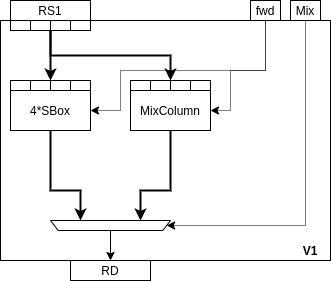
\includegraphics[width=\textwidth]{diagrams/ise-datapath-v1.png}
    \caption{Variant 1}
    \label{fig:design:fu_block:v1}
\end{subfigure}
\begin{subfigure}[t]{0.40\textwidth}
    \centering
    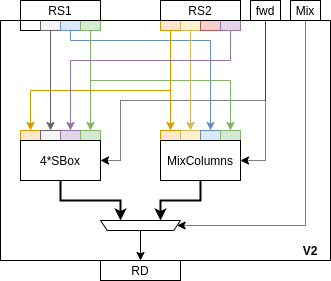
\includegraphics[width=\textwidth]{diagrams/ise-datapath-v2.png}
    \caption{Variant 2}
    \label{fig:design:fu_block:v2}
\end{subfigure}

\begin{subfigure}[t]{0.40\textwidth}
    \centering
    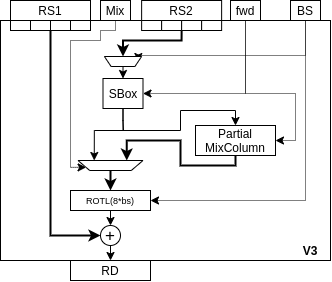
\includegraphics[width=\textwidth]{diagrams/ise-datapath-v3.png}
    \caption{Variant 3}
    \label{fig:design:fu_block:v3}
\end{subfigure}
\begin{subfigure}[t]{0.40\textwidth}
    \centering
    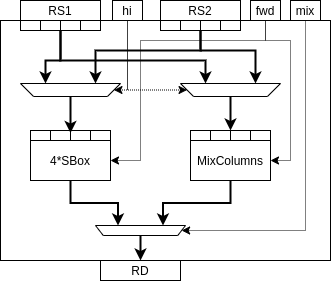
\includegraphics[width=\textwidth]{diagrams/ise-datapath-v5.png}
    \caption{Variant 5}
    \label{fig:design:fu_block:v5}
\end{subfigure}

\caption{
Micro-architecture block diagrams for the AES functional units, for
each ISE variant.
}
\end{figure}



\subsection{Variant $1$: column-wise acceleration}
\label{sec:design:v1}
% =============================================================================

\subsubsection{ISE interface}

% TODO: instruction definition(s)

% -----------------------------------------------------------------------------

\subsubsection{ISE implementation}

\begin{lstlisting}[language=pseudo,style=block]
saes.v1.encs(rs1):
    rd.8[i] =    SBox(rs1.8[i]) for i=0..3

saes.v1.decs(rs1):
    rd.8[i] = InvSBox(rs1.8[i]) for i=0..3

saes.v1.encm(rs1):
    rd.8[i] =    MixColumn(ROTL(rs1.32, 8*i))) for i=0..3

saes.v1.decm(rs1):
    rd.8[i] = InvMixColumn(ROTL(rs1.32, 8*i))) for i=0..3
\end{lstlisting}

% TODO: micro-architecture diagram

% =============================================================================


\subsection{Variant $2$: combined row/column acceleration}
\label{sec:design:v2}
% =============================================================================

\begin{figure}
\begin{subfigure}{\textwidth}
\begin{lstlisting}[language=pseudo,style=block]
saes.v2.encs rd, rs1, rs2 : v2.SubBytes(rd, rs1, rs2, fwd=1)
saes.v2.decs rd, rs1, rs2 : v2.SubBytes(rd, rs1, rs2, fwd=0)
saes.v2.encm rd, rs1, rs2 : v2.MixColumns(rd, rs1, rs2, fwd=1)
saes.v2.decm rd, rs1, rs2 : v2.MixColumns(rd, rs1, rs2, fwd=0)
\end{lstlisting}
\caption{
}
\label{fig:mnemonics:v2}
\end{subfigure}
\begin{subfigure}{\textwidth}
\begin{lstlisting}[language=pseudo,style=block]
lw              a0,  0(a4)     // Load Round Key
lw              a1,  4(a4)
lw              a2,  8(a4)
lw              a3, 12(a4)
xor             t0, t0, a0     // Add Round Key
xor             t1, t1, a1
xor             t2, t2, a2
xor             t3, t3, a3
saes.v2.sub.enc a0, t0, t1     // SubBytes / ShiftRows
saes.v2.sub.enc a1, t2, t3
saes.v2.sub.enc a2, t1, t2
saes.v2.sub.enc a3, t3, t0
saes.v2.mix.enc t0, a0, a1     // ShiftRows / MixColumns
saes.v2.mix.enc t1, a2, a3
saes.v2.mix.enc t2, a1, a0
saes.v2.mix.enc t3, a3, a2
\end{lstlisting}
\caption{
}
\label{fig:round:v2}
\end{subfigure}
\caption{
    Menmonics, pseudo code mappings and example encryption
    round function for variant 2.
    See \REFSEC{sec:pseudo}, \REFFIG{fig:pseudo:v2} for detailed
    descriptions of the pseudo-code functions.
}
\end{figure}

\REFFIG{fig:mnemonics:v2} shows the mnemonics and pseudo-code functions
for variant 2.
Here we reproduce the instructions proposed in Section $4.3$ of
\cite{TilGro:06}.
We continue to store the AES column-wise in $4$ $32$-bit words.
By using two source registers however,
the ShiftRows transformation can be implicitly performed by selecting
appropriate bytes from each source word.
\REFFIG{fig:design:fu_block:v2}
shows this.
Executing $4$  {\tt v2.encs}/{\tt v2.encm} instructions each hence
performs the entire SubBytes, ShiftRows and MixColumns steps.
The {\tt v2.encs} instruction can be used for the KeySchedule by
making {\tt rs1} equal to {\tt rs2}.

A single encryption round using this variant requires $16$ instructions
in total:
$4$ {\tt saes.v2.sub.enc} instructions to perform SubBytes and part of
shift rows,
$4$ {\tt saes.v2.mix.enc} instructions to perform MixColumns and the
remainder of shift rows,
$4$ load-word instructions to fetch the round key
and
$4$ {\tt xor} instructions to add the round key.
\REFFIG{fig:round:v2} shows an example AES encrypt round function
using this variant.

Because the final round does not include MixColumns, we must
complete the final ShiftRows operation with an additional
$12$ {\tt and}/{\tt or} instructions.

% =============================================================================


\subsection{Variant $3$: T-tables acceleration}
\label{sec:design:v3}
% =============================================================================

\subsubsection{ISE interface}

% TODO: instruction definition(s)

% -----------------------------------------------------------------------------

\subsubsection{ISE implementation}

\begin{lstlisting}[language=pseudo,style=block]
saes.v3.encs(rs1, rs2, bs):                 // SubBytes Only
    t0.8  = rs1.8[bs]
    x.8   = AESSBox(t0)
    u.32  = {0, 0, 0, x}
    rd.32 = ROTL32(u, 8*bs) ^ rs2.32

saes.v3.encsm(rs1, rs2, bs):                // SubBytes & MixColumns
    t0.8  = rs1.8[bs]
    x.8   = AESSBox(t0)
    u.32  = {GFMUL(x,3) , x, x, GFMUL(x,2)}
    rd.32 = ROTL32(u, 8*bs) ^ rs2.32

saes.v3.decs(rs1, rs2, bs):                 // InvSubBytes Only
    t0.8  = rs1.8[bs]
    x.8   = InvAESSBox(t0)
    u.32  = {0, 0, 0, x}
    rd.32 = ROTL32(u, 8*bs) ^ rs2.32

saes.v3.decsm(rs1, rs2, bs):                // InvSubBytes & InvMixColumns
    t0.8  = rs1.8[bs]
    x.8   = InvAESSBox(t0)
    u.32  = {GFMUL(x,11),GFMUL(x,13),GFMUL(9),GFMUL(14)}
    rd.32 = ROTL32(u, 8*bs) ^ rs2.32
\end{lstlisting}

% TODO: micro-architecture diagram

% =============================================================================


\subsection{Variant $4$: $64$-bit}
\label{sec:design:v4}
% =============================================================================

\subsubsection{ISE interface}

% TODO: instruction definition(s)

% -----------------------------------------------------------------------------

\subsubsection{ISE implementation}

\begin{lstlisting}[language=pseudo,style=block]
round_consts.8 = [0x01, 0x02, 0x04, 0x08, 0x10, 0x20, 0x40, 0x80, 0x1b, 0x36]

saes64.ks1(rs1,enc_rcon):      // KeySchedule: SubBytes, Rotate, Round Const
    temp.32   = rs1.32[1]
    rcon      = 0x0
    if(enc_rcon != 0xA):
        temp.32 = ROTR32(temp.32, 8)
        rcon    = round_consts.8[enc_rcon]
    temp.8[i] = AESSBox(temp.8[i])  for i=0..3
    temp.8[0] = temp.8[i  ] ^ rcon
    rd.64     = {temp.32, temp.32}

saes64.ks2(rs1,rs2):           // KeySchedule: XOR
    rd.32[0]  = rs1.32[1] ^ rs2.32[0]
    rd.32[1]  = rs1.32[1] ^ rs2.32[0] ^ rs2.32[1]

saes64.enc(rs1, rs2, mix, hi): // SubBytes, ShiftRows, MixColumns
    t1.128    = AESShiftRows(rs2 || rs1)
    t2.64     = t1.64[1] if hi else t1.64[0]
    t3.8[i]   = AESSBox(t2.8[i]) for i=0..7
    rd.32[0]  = AESMixColumn(t3.32[0]) if mix else t3.32[0]
    rd.32[1]  = AESMixColumn(t3.32[1]) if mix else t3.32[1]

saes64.dec(rs1, rs2, mix, hi): // InvSubBytes, InvShiftRows, InvMixColumns
    t1.128    = InvAESShiftRows(rs2 || rs1)
    t2.64     = t1.64[1] if hi else t1.64[0]
    t3.8[i]   = InvAESSBox(t2.8[i]) for i=0..7
    rd.32[0]  = InvAESMixColumn(t3.32[0]) if mix else t3.32[0]
    rd.32[1]  = InvAESMixColumn(t3.32[1]) if mix else t3.32[1]

saes64.imix(rs1):              // Inverse MixColumns
    rd.32[0]  = InvAESMixColumn(rs1.32[0])
    rd.32[1]  = InvAESMixColumn(rs1.32[1])
\end{lstlisting}

% TODO: micro-architecture diagram

% =============================================================================


\subsection{Variant $5$: tiled}
\label{sec:design:v5}
% =============================================================================
\begin{figure}
\begin{subfigure}{\textwidth}
\begin{lstlisting}[language=pseudo,style=block]
saes.v5.esrsub.lo rd, rs1, rs2 : rd = v5.SrSub(rs1, rs2, fwd=1, hi=0)
saes.v5.esrsub.hi rd, rs1, rs2 : rd = v5.SrSub(rs1, rs2, fwd=1, hi=1)
saes.v5.dsrsub.lo rd, rs1, rs2 : rd = v5.SrSub(rs1, rs2, fwd=0, hi=0)
saes.v5.dsrsub.hi rd, rs1, rs2 : rd = v5.SrSub(rs1, rs2, fwd=0, hi=1)
saes.v5.emix      rd, rs1, rs2 : rd = v5.Mix(rs1, rs2, fwd=1)
saes.v5.dmix      rd, rs1, rs2 : rd = v5.Mix(rs1, rs2, fwd=0)
saes.v5.sub       rd, rs1      : rd = SubBytes(rs1.8[i])         for i=0..3
\end{lstlisting}
\caption{}
\label{fig:mnemonics:v5}
\end{subfigure}
\begin{subfigure}{\textwidth}
\begin{lstlisting}[language=pseudo,style=block]
lw                a0,  0(a4)   // Load Round Key
lw                a1,  4(a4)
lw                a2,  8(a4)
lw                a3, 12(a4)
xor               t0, t0, a0   // Add Round Key
xor               t1, t1, a1
xor               t2, t2, a2
xor               t3, t3, a3
saes.v5.esrsub.lo a0, t0, t1   // Quad 0: SubBytes / ShiftRows
saes.v5.esrsub.lo a1, t1, t0   // Quad 1
saes.v5.esrsub.hi a2, t2, t3   // Quad 2
saes.v5.esrsub.hi a3, t3, t2   // Quad 3
saes.v5.emix      t0, a0, a2   // Quad 0: ShiftRows / MixColumns
saes.v5.emix      t1, a1, a3   // Quad 1
saes.v5.emix      t2, a2, a0   // Quad 2
saes.v5.emix      t3, a3, a1   // Quad 3
\end{lstlisting}
\caption{}
\label{fig:round:v5}
\end{subfigure}
\caption{
    Menmonics, pseudo code mappings and example encryption
    round function for variant 5.
    See \REFSEC{sec:pseudo}, \REFFIG{fig:pseudo:v5} for detailed
    descriptions of the pseudo-code functions.
}
\end{figure}

\REFFIG{fig:mnemonics:v5} shows the mnemonics and pseudo-code functions
for variant 5.
These instructions use a {\em tiled} approach to representing the
AES state.
Figure ({\bf TODO}) shows how the traditional column-wise representation
of AES is changed such that each {\em quadrant} of the 16-byte state
is kept in a single $32$-bit register.

We can now compute the next round state of any quadrant by sourcing
only two other quadrants (registers) at a time, thus keeping within
the $2$-read-$1$-write constraint.

The state matrix and must be re-arranged before and after applying
the round functions, which adds a small overhead to this variant.
Similarly, the KeySchedule words must also be re-arranged to allow
AddRoundKey to be performed efficiently.
This can be done as a post-processing step in the key expansion.

A single encryption round for this variant requires
$4$ load-word instructions to fetch the round key,
$4$ {\tt xor} instructions to perform AddRoundKey,
$4$ {\tt saes.v5.ersub.[lo|hi]} instructions to compute
    SubBytes, ShiftRows for each quadrant
and
$4$ {\tt saes.v5.emix} instructions to compute MixColumns for each
quadrant.
This would make it equivalent to variant 2, however we must also
account for the effort spent packing and un-packing the AES
state into the quadrant representation.
For the base ISA, this would take $12$ instructions to pack and
$12$ instructions to unpack the state.
We note that if the {\tt pack[h]} instructions from the draft
Bit-manipulation extension were included, then packing and unpacking
would be reduced to $4$ instructions.
\REFFIG{fig:round:v5} shows an example AES encrypt round function
using this variant.

% =============================================================================



% =============================================================================

\section{Evaluation}
\label{sec:eval}

\subsection{Host Cores}

The ISE designs were evaluated using two different {\em host} cores:

\begin{itemize}
\item
    The \CORE{2} core\footnote{%
  \ifbool{anonymous}{Details of this core have been anonymised to comply with the TCHES submission guidelines.}{\href{https://github.com/scarv/scarv-cpu}}
}   is a 5-stage, in-order scalar micro-controller.
    It implements the
    {\tt rv32imc}
    instruction set: 32-bit base ISA, with the Multiply and Compressed
    ISA extensions.
    A block diagram of the core is shown in~\REFFIG{fig:design:cpu_block:2}.
    The core has separate memory interfaces for instruction and data
    accesses, with no cache hierarchy or branch prediction.
    The core implements various performance counters,
    and
    elements of the
    RISC-V Privileged Resource Architecture 
    (PRA)~\cite[Chapter 3]{RV:ISA:II:17}
    related to exception and interrupt handling.

\item
    The \CORE{1} core\cite{rocket:16} 
    is a 5-stage, in-order pipeline with a configurable cache hierarchy and
    branch predictor.
    We used both 32-bit and 64-bit variants of \CORE{1} as bases for our work.
    We configured both base designs to have a single ``big" core, with
    no floating point support.
    ({\bf TODO:} List exactly how this configured Rocket)

\end{itemize}

Two modifications were made to the host cores to support the ISE variants:
1) The Instruction Decode module was modified to support identification and
   operand selection for the new instructions. 
2) A new ``AES" functional unit (AES FU) was added to perform the instruction
   computations.
In the \CORE{2} core, the new block was built directly into the execution
pipeline.
For the \CORE{1}, we used the Rocket Custom Coprocessor (RoCC)
interface.
Because all of the ISE variants read at most two,
and write one general purpose register, no new structural data-paths
were needed.
This was an important design consideration, as RISC-V tries to
aggressively follow this pattern.

All of the AES variants share the same sets of inputs, so the interface
to the AES FU is kept constant for every variant.
A synthesis time parameter was then added to switch between different
ISE variants for each host core.

The following sections give high level descriptions of the
instructions and their salient differences,
We list complete pseudo-code descriptions for each instruction
in the Appendix \REFSEC{sec:pseudo}.

\begin{figure}
\centering
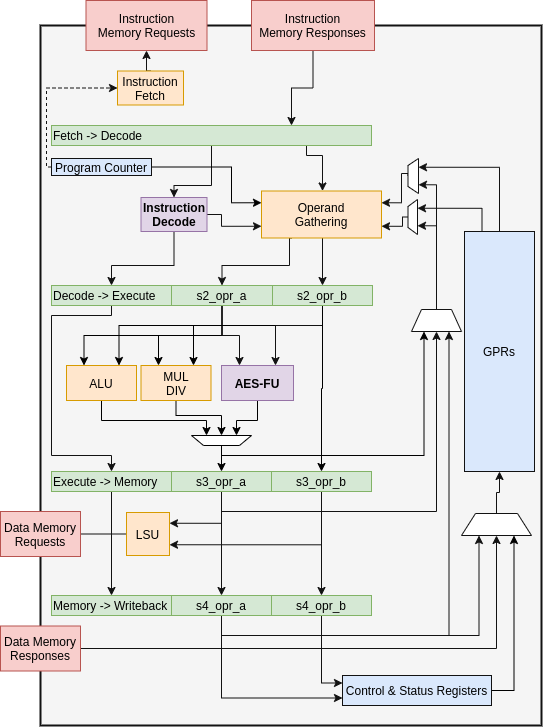
\includegraphics[scale=0.45,angle=90]{diagrams/scarv-cpu-uarch.png}
\caption{Core $2$: \CORE{2}.}
\label{fig:design:cpu_block:2}
\end{figure}

% =============================================================================

\subsection{Hardware Evaluation}
\label{sec:eval:sw}

Each ISE variant was evaluated on the host cores
described in \REFSEC{sec:design}.
The 32-bit designs (V1,V2,V3,V5) were implemented on both the
\CORE{1} and \CORE{2} cores.
The 64-bit design (v4) was only evaluated on the 64-bit configuration
of the \CORE{2} core.

Table \ref{tab:eval:hw}
shows the hardware implementation costs, while
Table \ref{tab:eval:sw}
shows performance and code size results for
each ISE, with software only versions of AES used as a baseline.

For variants 1, 2 and 5, two implementations are evaluated.
The ``Size" optimised implementations instantiate only a single
Forward/Inverse SBox and MixColumns circuit and take multiple cycles
to produce a result.
The ``Latency" optimised implementations instantiate $4$ SBox and
MixColumn circuits to produce their results in a single processor cycle.

The ISE Size column of Table \ref{tab:eval:hw} 
records the size in NAND2 equivalent gates of each variant,
instantiated independently from any wider system.
The LTP column gives the Longest Topological Path of the synthesised
functional unit circuit from input to combinatorial output.
The \CORE{2} Size column gives the size in NAND2 equivilent gates of the
\CORE{2}, with the various AES functional units integrated.
The ``Baseline" row gives the size of the core without any of the
ISEs integrated.
We found that none of the proposed ISEs affected the critical
path of the \CORE{2} core.

% ------------------------------------------------------------

\begin{table}
\centering
\begin{tabular}{lrrrr}
Variant     & ISE Size & ISE LTP & \CORE{2} Size & Size Overhead \\ \hline
Baseline    & -        & -       & 37375         & -             \\
V1 (Latency)& 3472     & 19      & 41723         & $  \%$        \\
V2 (Latency)& 3547     & 19      & 41199         & $  \%$        \\
V5 (Latency)& 4121     & 22      & 42070         & $  \%$        \\
V3          & 1157     & 30      & 38610         & $  \%$        \\
V4          &          &         &               & $  \%$        \\
V1 (Size)   & 2174     & 22      & 40161         & $  \%$        \\
V2 (Size)   & 1381     & 21      & 38885         & $  \%$        \\
V5 (Size)   & 1927     & 23      & 39251         & $  \%$        \\
\end{tabular}
\caption{
Hardware implementation costs based on the 32-bit \CORE{2} CPU core.
Gate counts and topological path lengths are obtained using the
Yosys\cite{yosys} tool suite.
}
\label{tab:eval:hw}
\end{table}



% =============================================================================


\subsection{Software Evaluation}
\label{sec:eval:sw}

To evaluate the software performance, we implemented AES 128, and
measure the static code size, instruction execution counts and cycle
counts of the Key Schedule, Encrypt and Decrypt functions.
We also separate generation of the KeySchedule for Encrypt and Decrypt.

\REFTAB{tab:eval:sw:size} shows the static code size for each
function.
We see that... ({\bf TODO}).

\REFTAB{tab:eval:sw:perf} gives cycle and instruction counts for each
variant.
Each implementation uses word-aligned state, meaning the input blocks
can be loaded with $4$ load-word instructions on $32$-bit host cores,
or $2$ load-double instructions on the $64$-bit host cores.

\begin{table}
\centering
\begin{tabular}{l|c|c|c|c|c}
Variant &
KeySchedule Enc  &
KeySchedule Dec  &
Encrypt Block    &
Decrypt Block    &
.data   \\ \hline
%Byte   & 312   &  -    &       &       & 522   \\
TTable  & 154   &  174  & 804   & 804   & 5120  \\
V1      & 68    &  -    & 424   & 424   & 10    \\
V2      & 68    &  62*  & 234   & 238   & 10    \\
V3      & 86    &  64   & 290   & 290   & 10    \\
V4      & 168   &  100  & 268   & 268   &  0    \\
V5      & 82+208&  -    & 266   & 278   & 10    \\
\end{tabular}
\caption{
Static code size metrics for each variant, measured in bytes.
These are measured targeting the {\tt rv32imc} base ISA for all variants,
except for V4, which targets {\tt rv64imc}.
}
\label{tab:eval:sw:size}
\end{table}


%
% Commented out this table because in the real world, you'd make sure that
% your state is well aligned!
%
% \begin{table}[pt]
% \centering
% \begin{tabular}{l|cc|cc|cc|cc}
% & \multicolumn{2}{c}{\begin{tabular}[c]{@{}c@{}}KeyExpand\\ Encrypt\end{tabular}} 
% & \multicolumn{2}{c}{\begin{tabular}[c]{@{}c@{}}KeyExpand\\ Decrypt\end{tabular}}
% & \multicolumn{2}{c}{\begin{tabular}[c]{@{}c@{}}AES 128\\ Encrypt\end{tabular}}
% & \multicolumn{2}{c}{\begin{tabular}[c]{@{}c@{}}AES 128\\ Decrypt\end{tabular}} \\
% Variant     &  iret & cycles & iret & cycles & iret & cycles & iret & cycles \\ \hline
%  Byte       &  926  & 3887   & 926  & 3886   & 4228 & 7061   & 7652 & 11587 \\
%  TTable     &  481  & 591    & 1762 & 2238   & 1013 & 1144   & 1013 & 1118  \\
% V1 (Latency)&  249  & 369    & 255  & 386    & 593  & 698    & 593  & 707   \\
% V2 (Latency)&  249  & 382    & 386  & 694    & 296  & 404    & 297  & 404   \\
% V3          &  269  & 388    & 719  & 1145   & 321  & 413    & 321  & 408   \\
% V5 (Latency)&  383  & 524    & 389  & 541    & 308  & 408    & 308  & 409   \\
% V1 (Size)   &  249  & 409    & 255  & 426    & 593  & 858    & 593  & 875   \\
% V2 (Size)   &  249  & 412    & 386  & 832    & 296  & 641    & 297  & 641   \\
% V5 (Size)   &  383  & 554    & 389  & 571    & 308  & 660    & 308  & 650   \\
% \end{tabular}
% \caption{
% Performance metrics for byte aligned state.
% }
% \label{tab:eval:sw:perf:byte}
% \end{table}

\begin{table}
\centering
\begin{tabular}{l|cc|cc|cc|cc}
& \multicolumn{2}{c}{\begin{tabular}[c]{@{}c@{}}KeySchedule\\ Encrypt\end{tabular}} 
& \multicolumn{2}{c}{\begin{tabular}[c]{@{}c@{}}KeySchedule\\ Decrypt\end{tabular}}
& \multicolumn{2}{c}{\begin{tabular}[c]{@{}c@{}}AES 128 Block\\ Encrypt\end{tabular}}
& \multicolumn{2}{c}{\begin{tabular}[c]{@{}c@{}}AES 128 Block\\ Decrypt\end{tabular}} \\
Variant     &  iret & cycles & iret & cycles & iret & cycles & iret & cycles \\ \hline
%Byte       & 926 & 3887 & 926 & 3886 & 4228 & 7061 & 7652 & 11587\\
 TTable     & 445 & 555 & 1726 & 2202 & 953 & 1078 & 953 & 1058   \\
V1 (Latency)& 213 & 333 & 219 & 350 & 533 & 635 & 533 & 647\\
V2 (Latency)& 213 & 344 & 350 & 656 & 236 & 343 & 237 & 343\\
V5 (Latency)& 347 & 489 & 353 & 506 & 248 & 346 & 248 & 349\\
V1 (Size)   & 213 & 373 & 219 & 390 & 533 & 795 & 533 & 815  \\
V2 (Size)   & 213 & 374 & 350 & 794 & 236 & 580 & 237 & 580  \\
V3          & 233 & 352 & 683 & 1109 & 261 & 351 & 261 & 346 \\
V5 (Size)   & 347 & 519 & 353 & 536 & 248 & 598 & 248 & 590  
\end{tabular}
\caption{
Performance results for the \CORE{2} core.
Note the absence of variant 4, as it is designed for 64-bit targets only.
}
\label{tab:eval:sw:perf:scarv}
\end{table}

\begin{table}
\centering
\begin{tabular}{l|cc|cc|cc|cc}
& \multicolumn{2}{c}{\begin{tabular}[c]{@{}c@{}}KeySchedule\\ Encrypt\end{tabular}} 
& \multicolumn{2}{c}{\begin{tabular}[c]{@{}c@{}}KeySchedule\\ Decrypt\end{tabular}}
& \multicolumn{2}{c}{\begin{tabular}[c]{@{}c@{}}AES 128 Block\\ Encrypt\end{tabular}}
& \multicolumn{2}{c}{\begin{tabular}[c]{@{}c@{}}AES 128 Block\\ Decrypt\end{tabular}} \\
Variant     &  iret & cycles & iret & cycles & iret & cycles & iret & cycles\\
\hline
%Byte       &       &        &      &        &      &        &       &      \\
 TTable     &       &        &      &        &      &        &       &      \\
V1 (Latency)&       &        &      &        &      &        &       &      \\
V2 (Latency)&       &        &      &        &      &        &       &      \\
V5 (Latency)&       &        &      &        &      &        &       &      \\
V1 (Size)   &       &        &      &        &      &        &       &      \\
V2 (Size)   &       &        &      &        &      &        &       &      \\
V3          &       &        &      &        &      &        &       &      \\
V4          &       &        &      &        &      &        &       &      \\
V5 (Size)   &       &        &      &        &      &        &       &     
\end{tabular}
\caption{
Performance results for the \CORE{1} core.
}
\label{tab:eval:sw:perf:scarv}
\end{table}

% ------------------------------------------------------------

We can see from the tables that ({\bf TODO}).

% =============================================================================


\subsection{Evaluation Discussion}
\label{sec:eval:results}

{\bf TODO:}
Note performance / unit area.
V3/ttable is the best canidate. Only one SBox, very fast per gate etc.


% =============================================================================

\section{Power Side-channel Resistance}
\label{sec:psca}

Many embedded implementations include power side-channels in their threat
model.
Having identified ISE variant $3$ detailed in
\REFSEC{sec:design:v3} as a strong candidate for embedded $32$-bit
RISC-V cores, we now show a possible
way of extending the ISE further to add power side-channel resistance
with minimal area and performance overheads.
We aim for $1$'st order side-channel security.

As described in \cite{TilGro:07}, there are several broad approaches
to adding power side-channel security to ISEs which we summarise here:

1) The data path can be implemented in a secure logic style, which always
consumes energy at the same rate, regardless of the values being computed on.
This comes with a significant overhead in terms of silicon area and
gate-level performance.
It also requires that secret values only be stored in secure logic
elements.
This can be undermined when loading keys from memory, since they must
pass through any register stages in the memory hierarchy, which are
unlikely to be implemented in a secure logic style.

2) Random pre-charging involves sandwiching every instruction which
manipulates a secret value with instructions which operate on random values.
As the authors of \cite{TilGro:07} note, it provides only a modest
improvement in security, and comes with a $100\%$ performance overhead;
since every secret manipulating instruction must be accompanied by
a random-pre-charging partner.

3) The authors also describe a small ``secure zone'' within the processor,
implemented in a secure logic style and responsible for
mask storage, generation and all computations on secret data.
The aim is to keep the secure zone as small and separate from the main
processor data-path as possible.

\subsection{Design Overview}

We extend ISE variant $3$ to support 1'st order masking.
To this end, the secret key is represented as two boolean masked shares.
An implementation of the AES block encrypt/decrypt function requires
eight registers: four for the current round state, four to load the
next round key into and then accumulate the next round state.
Doubling this requirement to store shares of each secret variable
in the General Purpose Register (GPR) file is un-reasonable.
It would require drastic modifications to the instruction definitions and
register file to read four registers (two sources, of two shares each) and
write two registers.

Instead, we define a new, $8$-element ``Mask Register File'' (MRF).
Each mask register $M_i$ is $32$-bits wide, and stores the mask for
one of the GPRs.
We use a fixed mapping between GPRs and mask registers;
not all GPRs have a corresponding mask register.
({\bf TODO:} define this mapping. E.g. \{a0..a3,t0..t4\} onto MRF \{0..7\}).

Share $0$ of each secret value is loaded into the GPRs.
We define a new Load Mask instruction {\tt lm rd, imm(rs1)} which
loads {\em the mask for GPR {\tt rd}} from memory into the MRF.
A corresponding Store Mask instruction {\tt sm rs2, imm(rs1)} writes
the mask corresponding to GPR {\tt rs2} to memory.
We require that the secret values be stored in shared form in memory
(rather than splitting them into shares upon being loaded)
to extend the SCA protection boundary outside the CPU.
Otherwise, the hamming weight of un-masked secret values would be
leaked by memory-hierarchy registers outside the CPU.

When an ISE instruction is executed such that any of its GPR source
registers also map onto an MRF register, both GPR and MRF are
read simultaneously and fed to the AES functional unit.
If any GPR source does not map to an MRF register, we assume that
operand is un-masked and represent the other share as $0$.

Within the AES FU the instruction result is computed entirely in it's
masked representation.

The result is re-masked using a randomness source.

Share 0 goes to GPR, Share 1 to the MRF.

If destination is not a GPR, result is written back un-masked.


% =============================================================================

\section{Conclusion}
\label{sec:outro}
% =============================================================================

{\bf TODO:}

% =============================================================================


% ============================================================================

\ifbool{anonymous}{}{%
\section*{Acknowledgements}

We would like to thank the anonymous reviewers for their helpful and 
constructive comments.
This work has been supported in part by EPSRC via grant EP/R012288/1, 
under the RISE (\url{http://www.ukrise.org}) programme.
}%

% =============================================================================

\bibliographystyle{alpha}
\bibliography{paper}

% =============================================================================

\appendix

\section{ISE Instruction Pseudo Code}
\label{sec:pseudo}

%
% V1
% ------------------------------------------------------------

\begin{figure}[!htb]
\begin{lstlisting}[language=pseudo,style=block]
v1.SubByte(rd, rs1, fwd):
    rd.8[i] = AESSBox[rs1.8[i]] if fwd else AESInbSBox[rs1.8[i]] for i=0..3

v1.MixColumn(rd, rs1, fwd)
    for i=0..3:
        tmp.32  = ROTL32(rs1.32, 8*i)
        rd.8[i] = AESMixColumn(tmp.32) if fwd else AESInvMixColumn(tmp.32)
\end{lstlisting}
\caption{
    Variant 1 psuedo code.
    See section \REFSEC{sec:design:v1} for the instruction
    descriptions.
}
\label{fig:pseudo:v1}
\end{figure}

%
% V2
% ------------------------------------------------------------

\begin{figure}[!htb]
\begin{lstlisting}[language=pseudo,style=block]
v2.SubBytes(rd, rs1, rs2, fwd):
  t1.32  = {rs1.8[0], rs2.8[1], rs1.8[2], rs2.8[3]}
  rd.8[i]= AESSBox[t1.8[i]] if fwd else AESInvSBox[t1.8[i]] for i=0..3

v2.MixColumns(rd, rs1, rs2, fwd):
  t1.32  = {rs1.8[0], rs1.8[1], rs2.8[2], rs2.8[3]}
  for i=0..3:
      tmp.32 = ROTL32(rs1.32, 8*i)
      rd.8[i]= AESMixColumn(tmp.32) if fwd else AESInvMixColumn(tmp.32)
\end{lstlisting}
\caption{
    Variant 2 psuedo code.
    See section \REFSEC{sec:design:v2} for the instruction
    descriptions.
}
\label{fig:pseudo:v2}
\end{figure}

%
% V3
% ------------------------------------------------------------

\begin{figure}[!htb]
\begin{lstlisting}[language=pseudo,style=block]
v3.Proc(rd, rs1, rs2, bs, fwd, mix):
  x     = AESSBox[rs2.8[bs]] if fwd else AESInvSBox[rs2.8[bs]]
  if   mix and  fwd: t1.32 = {GFMUL(x, 3),      x    ,      x   ,GFMUL(x, 2)}
  elif mix and !fwd: t1.32 = {GFMUL(x,11),GFMUL(x,13),GFMUL(x,9),GFMUL(x,14)}
  else             : t1.32 = {0, 0, 0, x}
  rd.32 = ROTL32(t1.32, 8*bs) ^ rs1
\end{lstlisting}
\caption{
    Variant 3 psuedo code.
    See section \REFSEC{sec:design:v3} for the instruction
    descriptions.
}
\label{fig:pseudo:v3}
\end{figure}

%
% V4
% ------------------------------------------------------------

\begin{figure}[!htb]
\begin{lstlisting}[language=pseudo,style=block]
v4.ks1(rd, rs1, enc_rcon):     // KeySchedule: SubBytes, Rotate, Round Const
    temp.32   = rs1.32[1]
    rcon      = 0x0
    if(enc_rcon != 0xA):
        temp.32 = ROTR32(temp.32, 8)
        rcon    = RoundConstants.8[enc_rcon]
    temp.8[i] = AESSBox[temp.8[i]]  for i=0..3
    temp.8[0] = temp.8[0] ^ rcon
    rd.64     = {temp.32, temp.32}

v4.ks2(rd, rs1, rs2):           // KeySchedule: XOR
    rd.32[0]  = rs1.32[1] ^ rs2.32[0]
    rd.32[1]  = rs1.32[1] ^ rs2.32[0] ^ rs2.32[1]

v4.Enc(rd, rs1, rs2, mix): // SubBytes, ShiftRows, MixColumns
    t1.128    = ShiftRows({rs2, rs1})
    t2.64     = t1.64[0]
    t3.8[i]   = AESSBox[t2.8[i]] for i=0..7
    rd.32[i]  = AESMixColumn(t3.32[i]) if mix else t3.32[i] for i=0..1

v4.Dec(rd, rs1, rs2, mix, hi): // InvSubBytes, InvShiftRows, InvMixColumns
    t1.128    = InvShiftRows(rs2 || rs1)
    t2.64     = t1.64[0]
    t3.8[i]   = AESInvSBox[t2.8[i]] for i=0..7
    rd.32[i]  = AESInvMixColumn(t3.32[i]) if mix else t3.32[i] for i=0..1

v4.InvMix(rd, rs1):             // Inverse MixColumns
    rd.32[i]  = AESInvMixColumn(rs1.32[i]) for i=0..1
\end{lstlisting}
\caption{
    Variant 4 psuedo code.
    See section \REFSEC{sec:design:v4} for the instruction
    descriptions.
}
\label{fig:pseudo:v4}
\end{figure}

%
% V5
% ------------------------------------------------------------

\begin{figure}[!htb]
\begin{lstlisting}[language=pseudo,style=block]
v5.SrSub(rd, rs1, rs2, fwd, hi):
  if(fwd):
    if hi: tmp.32 = {rs1.8[3], rs2.8[0], rs2.8[1], rs2.8[2]}
    else : tmp.32 = {rs2.8[3], rs1.8[1], rs1.8[0], rs1.8[2]}
    tmp.8[i]      =    AESSBox[tmp.8[i]] for i=0..3
  else:
    if hi: tmp.32 = {rs2.8[3], rs2.8[0], rs1.8[1], rs2.8[2]}
    else : tmp.32 = {rs1.8[3], rs2.8[1], rs1.8[0], rs1.8[2]}
    tmp.8[i]      = InvAESSBox[tmp.8[i]] for i=0..3
  if(hi): rd.32 = {tmp.8[2],tmp.8[3],tmp.8[0],tmp.8[1]}
  else  : rd.32 = {tmp.8[1],tmp.8[3],tmp.8[0],tmp.8[2]}

v5.mix(rd, rs1, rs2, fwd):
  col0.32 = {rs1.8[2], rs1.8[3], rs2.8[2], rs2.8[3]}
  col1.32 = {rs1.8[0], rs1.8[1], rs2.8[0], rs2.8[1]}
  n0.8    = AESMixColumn(       col0   ) if fwd else AESInvMixColumn(       col0   )
  n1.8    = AESMixColumn(ROTL32(col0,8)) if fwd else AESInvMixColumn(ROTL32(col0,8))
  n2.8    = AESMixColumn(       col1   ) if fwd else AESInvMixColumn(       col1   )
  n3.8    = AESMixColumn(ROTL32(col1,8)) if fwd else AESInvMixColumn(ROTL32(col1,8))
  rd.32 = {n2, n3, n0, n1}
\end{lstlisting}
\caption{
    Variant 5 psuedo code.
    See section \REFSEC{sec:design:v5} for the instruction
    descriptions.
}
\label{fig:pseudo:v5}
\end{figure}



% =============================================================================

\end{document}
